\documentclass{article}
\usepackage{hyperref}
\usepackage{booktabs}
\usepackage{float}
\usepackage{url}
\usepackage{graphicx}
%\usepackage{geometry}
\usepackage[a4paper, left=0.8in, right=0.8in, top=1in, bottom=1in]{geometry}
\usepackage{longtable}


% Title Information
\title{Values Encoded in Machine Learning Research}
\author{Isabel Kurth\thanks{Hasso Plattner Institute, Potsdam, Germany.\ \texttt{isabel.kurth@student.hpi.de}}}

% Document Start
\begin{document}

\maketitle
\thispagestyle{plain}

% Abstract Section
\begin{abstract}
% \textbf{Keywords:} Machine Learning, Ethics, Values, Society, Impact
\end{abstract}

% Sections
\section{Introduction}
Machine learning (ML) research has become a driving force behind technological advancements across diverse domains, including healthcare \cite{esteva2019guide}, finance \cite{berg2022fintech}, and autonomous systems \cite{hawkins2021guidance}. 
However, despite its transformative potential, the values embedded in ML research remain underexamined, 
raising critical questions about whom the field serves and whose needs it prioritizes. The previous study by Birhane et al. \cite{valuesInML2021} has demonstrated that ML research overwhelmingly prioritizes 
performance, generalization, and novelty while often neglecting ethical considerations, fairness, and broader societal impacts.

In this work, we build upon the foundational analysis by Birhane et al., extending the study to the most influential papers from NeurIPS 2023 and ICML 2023. 
These conferences represent the cutting edge of ML research and serve as key venues where emerging trends and priorities become crystallized. By systematically analyzing these highly-cited papers, 
we aim to uncover the prevailing value commitments in ML research and assess whether the field has shifted its focus towards more socially responsible AI.

Our methodology involves a keyword-based analysis, complemented by qualitative reviews, to measure the prevalence of ethical and performance-driven values in recent ML research. While previous studies \cite{geyik2019fairness} 
have emphasized the need for fairness-aware ML, our findings indicate that technical considerations such as state-of-the-art (SOTA) performance and computational
efficiency continue to dominate, often at the expense of user rights and transparency.
This study contributes to the growing discourse on the socio-political dimensions of ML research by providing empirical insights into the values upheld in contemporary work. By situating our findings within 
the broader ML ethics literature, we aim to encourage researchers, institutions, and policymakers to critically reflect on the long-term implications of prioritizing 
certain values over others. Our analysis reveals a pressing need to reorient ML research towards more equitable and inclusive technological development, aligning with calls for ethical AI \cite{floridi2022unified}, \cite{kalluri2020don}

\section{Methodology}
\subsection{Data collection}
We curated a dataset of the 100 most influential papers from NeurIPS 2023 and ICML 2023 using rankings provided by Paper Digest 
(\url{https://www.paperdigest.org/topic/?topic=nips&year=2023} and \url{https://www.paperdigest.org/topic/?topic=icml&year=2023}). 
These rankings were based on an impact score, which reflects a combination of paper citations, patent citations, etc. It is a score in 1.0-10.0, 
with a higher value indicating a broader impact. We then downloaded the respective papers from the conference website directly 
(\url{https://proceedings.neurips.cc/paper_files/paper/2023} and \url{https://icml.cc/Downloads/2023}). 
The selected papers represent the cutting edge of machine 
learning research and provide a representative sample of current trends and values in the field. We did not use Semantic Scholar as in the Birhane et 
al. (2023) paper because Semantic Scholar did not provide API keys due to high demand. We could also not use Google Scholar to access the citation 
counts because the IP address gets blocked after too many access tries. A list of the PDFs of the 100 papers of both conferences can be found in the 
GitHub repository: \url{https://github.com/IsabelKurth/values-in-ml-research}.

\subsection{Keyword based analysis}
To analyze the values encoded in these papers, we adopted the 74 keywords used by Birhane et al. (2023) in their study of influential ML papers. In their paper
they write that they use 67 values, but in their annotation template for manual annotations (annotations.tsv) they include 74 values. In their results folder they
just mention 62 values. In order to search for as many values as possible we decided to proceed with the 74 values from the annotation file in their data folder.  
These keywords include terms related to performance, generalization, novelty, societal impact, and ethical considerations. 
Unlike Birhane et al., who relied on manual annotation, we developed and deployed an automated keyword-scanning algorithm to systematically identify the presence of 
these keywords across the abstracts, introductions, and conclusions of the selected papers.
The Table\ref{tab:keyword_table} in the Appendix provides a comprehensive list of the values and their associated keywords used in our analysis.
For example we did not only query for the additonal keyword ``Novelty'' but also for ``novel'' as these two
words express the same value and because we use a keyword search, sentences with the word ``novel'' would not be counted towards the keyword ``Novelty''.  
For each keyword occurrence, contextual information was extracted to ensure accurate interpretation. 
This semi-automated process balanced the scale of automated analysis with the depth of manual review. One major limitation to this keyword based approach is 
that for some keywords this works better than for others and these keywords might then be under- or overrepresented in the analysis. For example for the keyword ``Fairness'' is 
is really likeli that the keyword search will find the occurences if the paper adresses this topic because they will most liekli use the word in the context. 
As a counter example the keyword `Èasy to implement'' might not be found as easily because the word ``easy'' is used in many other contexts as well and therefore we can not query for it.
There are many different words in witch the researchers could express that their model is easy to implement and they are hard to capture all by a simple keyword search. In order to keep that limitations as simple as possible
we try to query for many similar keywords and hope that this will cover most of the values.
Even tough the keyword search is not perfect, it is a good way to get a first overview of the values encoded in the papers and to get a first impression of the values. To stay in the scope of this seminar paper 
we therefor decided to use this approach but we want to explicitly mention this limitation.

\subsection{Quantitative Summary}
We measure the prevelence of each keyword in the 100 papers from the ICML 2023 conference and the 100 papers from the NeurIPS 2023 conference. First we investigate the combined distribution of the keywords in both conferences, second we look at both conferences seperately,
and lastly we compare the results from the 2023 papers with the results from the 2008/09 and 2018/19 papers from Birhane et al. \cite{valuesInML2021}. 
In line with the Birhane et al. paper we highlight the values that fall under `User rights'. These are `Interpretable (To Users)', `Deferral To Humans', `Privacy', `User influence', `Not Socially Biased' and `Fairness'. 
These values are highlighted in all plots in orange. The second group of values highlighted are values belonging to `Ethical Principles', These keywords are `Beneficence', `Non-Maleficence', `Respect for Law and Public Interest', 
`Respect for Persons', `Autonomy (Power to Decide)', `Explicability' and `Justice'.
\subsubsection{ICML and Neurips 2023}
In Figure \ref{fig:percentage_both_conferences} we show the prevelance of values in all 200 papers combined from ICML and Neurips 2023. The top values are performance (99\%), accuracy (85\%), 
Understanding (for researchers) (82.5\%), Efficiency (81\%) and Fast (80\%). Among the values related to user rights and stated in 
ethical principles the most common ones are `Explicability' (22.5\%) and Privacy (21.5\%). 

\begin{figure}[H]
    \centering
    %\hspace{-2cm}
    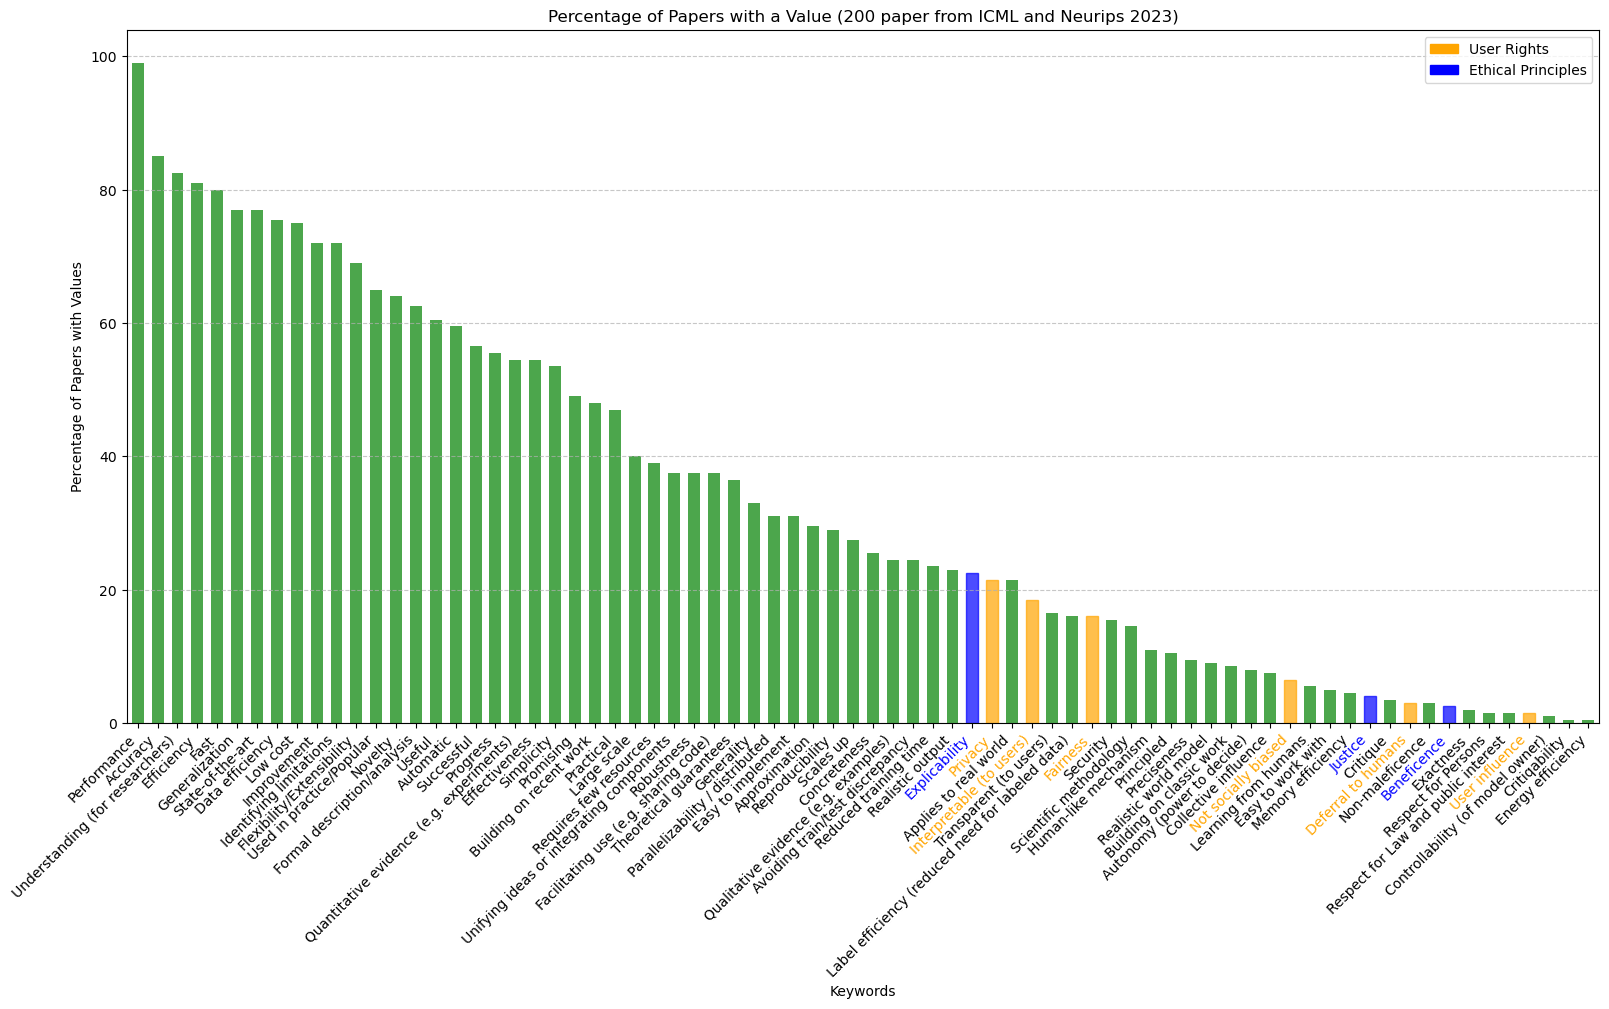
\includegraphics[width=\textwidth]{../plots/percentage_both_conferences.png}
    \caption{Prevalence of values in the 200 most influential papers from ICML 2023 and NeurIPS 2023. Values related to user rights are highlighted in orange, and values belonging to ethical principles are highlighted in blue.}
    \label{fig:percentage_both_conferences}
\end{figure}

By analysing the 100 most influencial paper from both conferences seperately we can see in Figure \ref{fig:percentage_comparison_conferences}
that the distribution of values are quite similar in both conferences. The top values in both conferences are performance, accuracy, understanding (for researchers), efficiency and fast.
that the maximum length for a paper is nine pages for Neurips (\url{https://neurips.cc/Conferences/2023/PaperInformation/NeurIPS-FAQ}) and only eight pages for ICML (\url{https://icml.cc/Conferences/2023/StyleAuthorInstructions}). If the paper
are shorter the possibility of including values drops due to the space limitation. 
\begin{figure}[H]
    \centering
    
\includegraphics[width=\textwidth]{../plots/percentage_comparison_conferences.png}
    \caption{Comparison of prevalence of values in the 200 most influential papers from ICML 2023 and NeurIPS 2023. Values related to user rights are highlighted in orange, and values belonging to ethical principles are highlighted in blue.}
    \label{fig:percentage_comparison_conferences}
\end{figure}


These plots always show the percentage of papers that contain the specific value. In order to take into account if one value is detected multiple times in a paper. We can see in Figure \ref{fig:total_counts }the total counts of the values in the papers
for both conferences. This emphasises that Performance is by far the most addressed value in the papers. 
\begin{figure}[H]
    \centering
    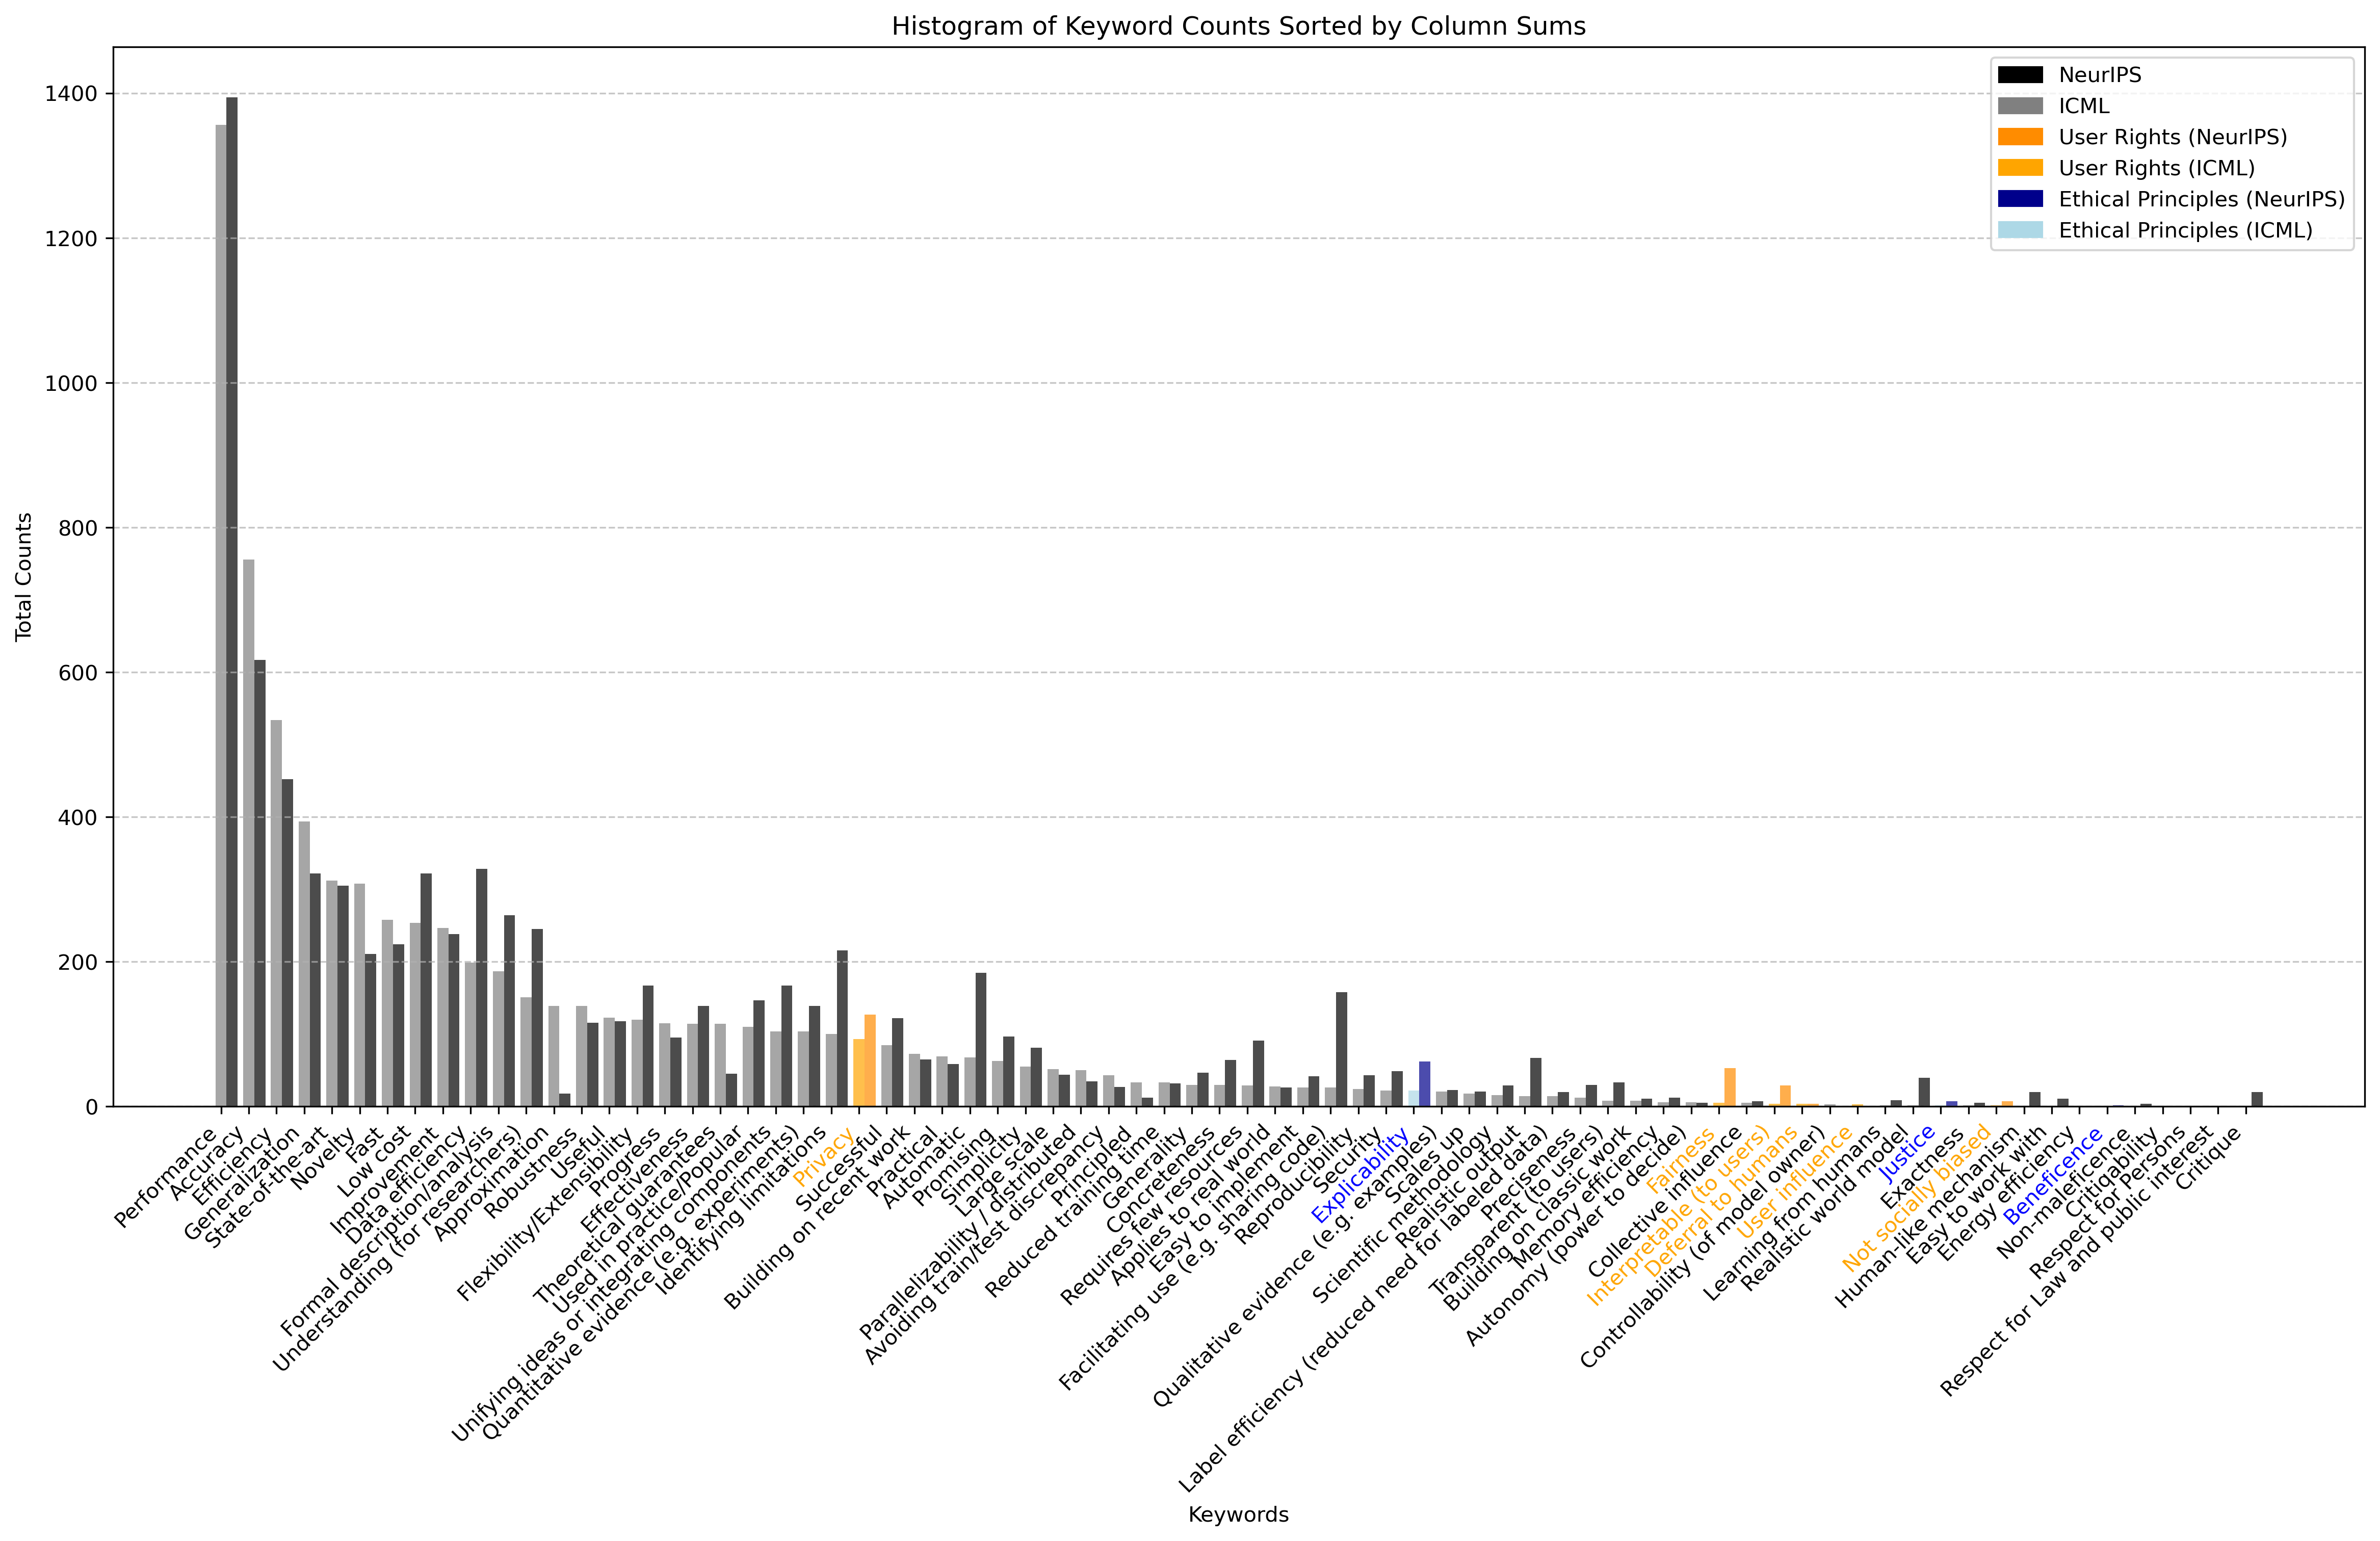
\includegraphics[width=\textwidth]{../plots/histogram_keyword_counts_total_number.png}
    \caption{Comparison of total counts of the Values.}
    \label{fig:total_counts}
\end{figure}

\subsubsection{Comparison 2008/09 and 2018/19 to 2023}
In Figure \ref{fig:percentage_comparison_years} we compare the distribution of values in the 200 most influential papers from ICML 2023 and NeurIPS 2023 with the results from Birhane et al.
There are a few values that have a high percentage in both the 2023 papers and the papers from 2008/09 and 2018/19. 
These are performance (2023: 99\% and Brihane: 96\%), generalisation(77\% and 89\%) and efficiency (81\% and 84\%). 
\begin{figure}[H]
    \centering
    
\includegraphics[width=\textwidth]{../plots/percentage_comparison_brihane.png}
    \caption{Comparison of prevelance of values from 2023 to 08/09 and 18/19 from Brihane et al.}
    \label{fig:percentage_comparison_years}
\end{figure}
Strong differences as in values such as `Automatic' and `Progress' can potentially be explaind due to the fact that these 
words occur often also without specific meaning towards the values. 

By looking closer at the values related to user rights and ethical principles in Figure \ref{fig:subset_comparison_years}
we can see an increase in the percentage of papers with these values from 2008/09 and 2018/19 to 2023 expect for `Deferral to humans' and `User influence'. Here the 
decrease is so small that it could also be due to the keyword search. Especially in the values `Privacy' and `Explicability' we see and strong increase. 
\begin{figure}[H]
    \centering
    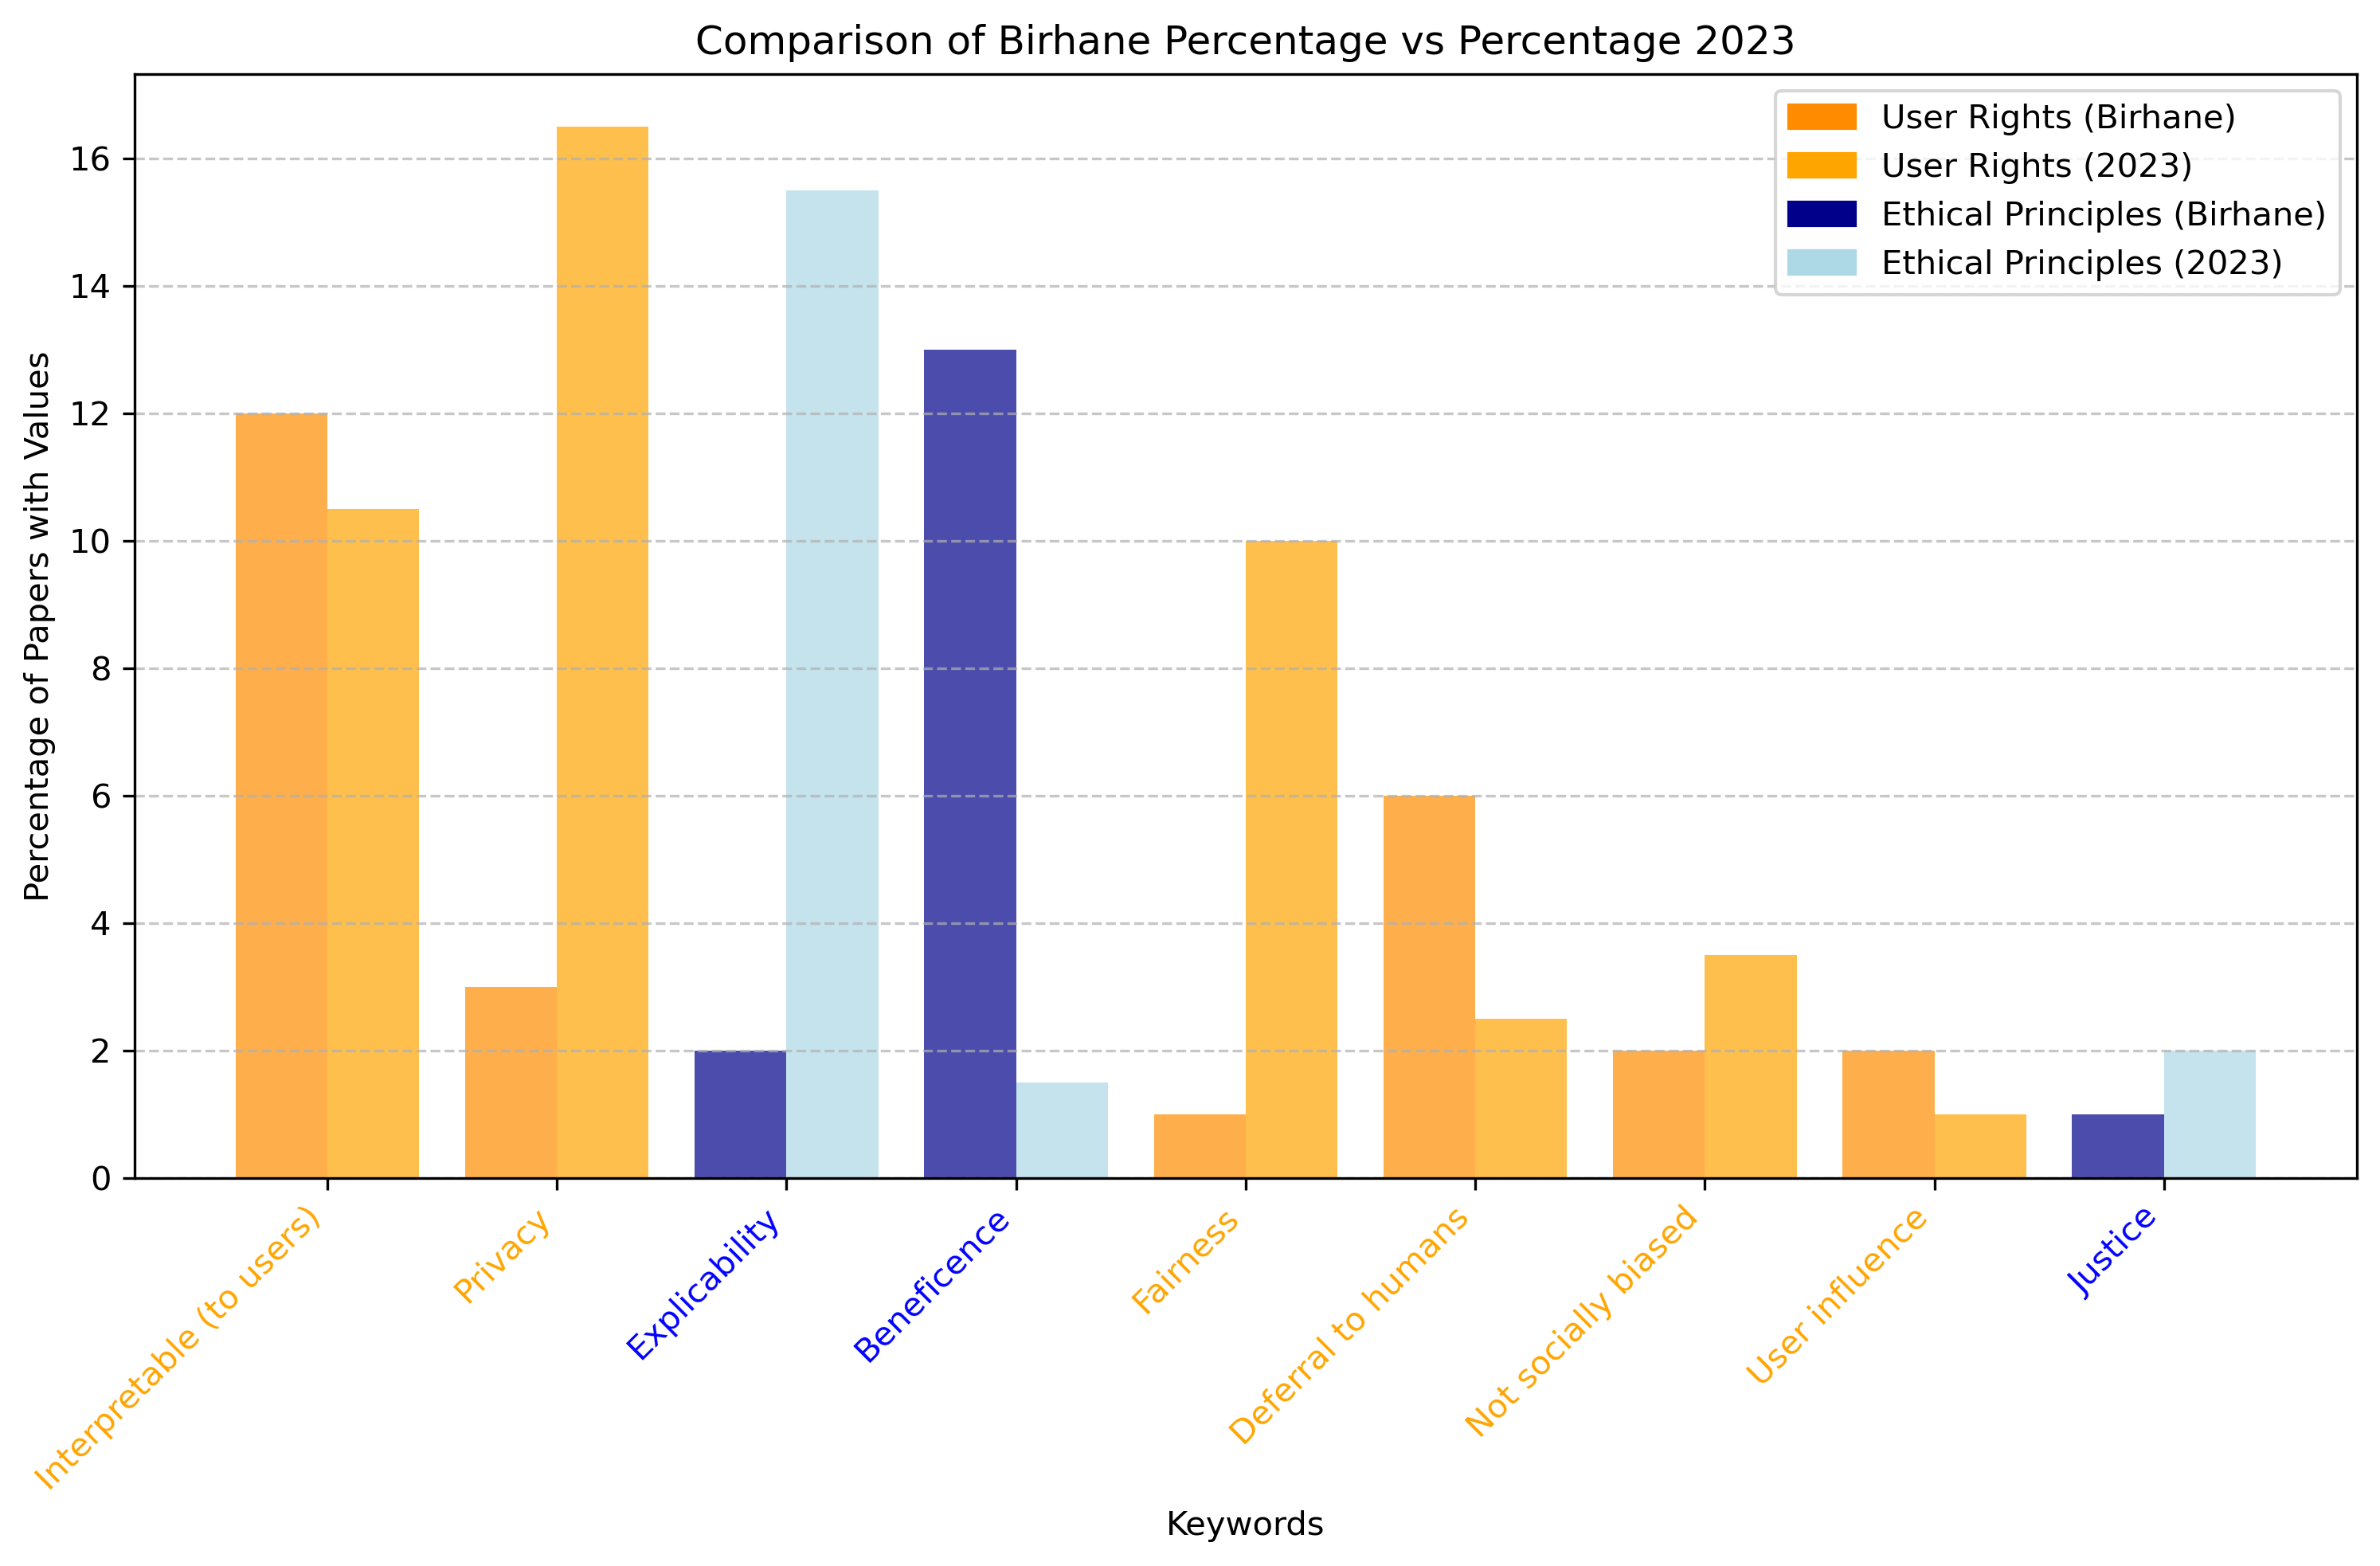
\includegraphics[width=0.8\textwidth,height=0.32\textheight]{../plots/subset_percentage_comparison.png}
    \caption{Comparison of values related to user rights and to ethical principles.}
    \label{fig:subset_comparison_years}
\end{figure}

\subsection{Qualitative Summary}
In order to investigate if the keyword search was able to capture values correctly, we manually review 
the sentences flagged for specific values. This qualitative analysis provides a nuanced understanding of how values are encoded in the papers. 
Table \ref{tab:qualitative_examples_user_influence} provides examples of sentences from the papers that reflect the value `User influence'. These
examples show that by the automated keywords search in this case sentences get flagged that actually stand in context with the value. 
\begin{table}[H]
    \centering
    \begin{tabular}{p{12cm}}
        \toprule
        ``However, in contrast to existing works that target a specific application, without a well defined objective, we propose a more general approach that allows us to unify different user control inputs in a more principled manner.'' \\
        \midrule
        ``Controllable Diffusion Models are designed to enable T2I diffusion models to accept more user controls for guiding the generation results.'' \\
        \midrule
        ``Recently, a surge of methods have been proposed to gain wider and better user controllability.'' \\
        \bottomrule
    \end{tabular}
    \caption{Random examples of the value \textit{User influence} in the context.}
    \label{tab:qualitative_examples_user_influence}
\end{table}

For the values `Fairness' we can see in Table \ref{tab:qualitative_examples_fairness} that the keyword search was able to capture the values correctly in the first two example sentences.
In the last case the automated search did wrongly also flag a reference cited in the paper that was publsiehd at the ACM COnference on Fairness, Accountability, and Transparency. 
In this case the value fairness was not part of the paper but it got flagged. This shows a limitation of the automated appraoch. 


\begin{table}[H]
    \centering
    \begin{tabular}{p{12cm}}
        \toprule
        ``In scenario ( 1), Table 4 shows the fairness issues of GPT-3.5 and GPT-4.'' \\
        \midrule
        ``It is unclear whether other properties that have been extensively studied in the literature for the existing public BERT checkpoint, such as robustness, out-of-distribution generalization, fairness or inherent biases, carry over to the crammed model.'' \\
        \midrule
        ``In 2022 ACM Confer- ence on Fairness, Accountability, and Transparency , pp.'' \\
        \bottomrule
    \end{tabular}
    \caption{Random examples of the value \textit{Fairness} in the context.}
    \label{tab:qualitative_examples_fairness}
\end{table}

We provide in the code the possibility to search for the values the reader is most interested in and one gets 
as output the names of the paper and the sentences that got flagged. 

\section{Discussion}
Our study extends the analysis of values encoded in machine learning (ML) research by examining the most influential papers from NeurIPS 2023 and ICML 2023. In alignment with prior work by Birhane et al. (2023), 
we find that performance, accuracy, generalization, and efficiency remain dominant values in contemporary ML research. However, our findings also suggest an increasing emphasis on ethical considerations, particularly 
explicability and privacy, indicating a growing awareness of the societal implications of ML advancements.
A key observation in our study is that the priorities of ML research largely remain entrenched in technical performance metrics. The emphasis on state-of-the-art (SOTA) performance and efficiency continues to drive the field, 
yet the explicit inclusion of values related to fairness, transparency, and social responsibility remains relatively limited. While there is a slight increase in the prevalence of values associated with user rights, such as 
privacy and explicability, these considerations are still secondary to performance-driven objectives. This reinforces concerns raised by Birhane et al. (2023) that ML research prioritizes technical achievements over broader 
social impact.
The keyword-based methodology we employed, while effective for large-scale analysis, introduces limitations regarding contextual accuracy. Automated searches for ethical principles may fail to capture nuanced discussions, 
as seen in cases where references to fairness or accountability appeared only in citations rather than substantive discourse. This underscores the need for complementary qualitative analysis to provide deeper insights into 
the way these values are operationalized in ML research.

\section{Conclusion}
Our analysis reveals that while ML research is increasingly acknowledging ethical concerns such as privacy and explicability, technical performance metrics continue to dominate. 
The persistence of values such as performance, efficiency, and generalization, while important for technological progress, indicates that broader social considerations remain underprioritized. 
Despite the growing discourse around fairness, transparency, and ethical AI, these values are not yet as deeply embedded in ML research as one might hope.

This study underscores the need for a more deliberate integration of ethical principles into ML research. Future work should explore alternative evaluation metrics that balance technical performance 
with social responsibility. Moreover, institutions and funding bodies should incentivize research that explicitly addresses societal needs, ensuring that ML advancements contribute to equitable and 
inclusive technological progress.

Finally, our findings highlight the importance of methodological rigor in value analysis. While keyword-based approaches provide valuable quantitative insights, they must be supplemented with 
qualitative evaluations to accurately capture the nuances of how values are expressed in ML research. As ML continues to shape critical aspects of society, ongoing scrutiny of the values encoded in its 
research will be essential for fostering responsible and equitable AI development.




% References
\bibliographystyle{plain}
\bibliography{references}

% Appendix
\appendix

\section{Keyword Analysis Table}

\begin{longtable}{|p{5cm}|p{10cm}|} 
    \caption{Values and their associated keywords used in the analysis.} \\
    \hline
    \textbf{Keywords Birhane Paper} & \textbf{Additional Keywords for Automated Search} \\
    \hline
    \endfirsthead

    \hline
    \textbf{Keywords Birhane Paper} & \textbf{Additional Keywords for Automated Search} \\
    \hline
    \endhead
    
    % Table content
    Novelty & novel, innovative, groundbreaking \\ 
    Simplicity & minimalistic, concise, parsimonious \\ 
    Generalization & generalisable, generalizable, transferability \\ 
    Flexibility/Extensibility & flexible, flexibility, extensibility, extensible, adaptable, modular, scalable \\ 
    Robustness & resilient, fault-tolerant, noise tolerance \\ 
    Realistic output & authentic, plausible \\ 
    Formal description/analysis & formal, mathematical, rigorous, analytical, axiomatic, proof-based \\ 
    Theoretical guarantees & guarantee, provable, convergence proof, theoretical bound, performance bound \\ 
    Approximation & approximation theory \\ 
    Quantitative evidence & quantitative, numerical results, empirical study, measurable \\ 
    Qualitative evidence & case study, illustrative \\ 
    Scientific methodology & hypothesis-driven, scientific \\ 
    Controllability (of model owner) & governability, ownership, model steering \\ 
    Human-like mechanism & biologically inspired, cognitive \\ 
    Low cost & cheap, cost, affordable, resource-efficient, budget-friendly \\ 
    Large scale & scalability, big data, high-capacity, massive-scale \\ 
    Promising & \\ 
    Generality & broad applicability, domain-independent, versatile \\ 
    Principled & theoretically sound, axiomatic, methodologically rigorous \\ 
    Exactness & error-free \\ 
    Preciseness & high-fidelity \\ 
    Concreteness & grounded, verifiable \\ 
    Automatic & self-operating, hands-free \\ 
    Performance & \\ 
    Accuracy & precision, recall, F1-score, error rate, reliability \\ 
    Avoiding train/test discrepancy & train/test, discrepancy, distribution shift, generalization gap \\ 
    State-of-the-art & SOTA, best performing, cutting-edge, latest \\ 
    Efficiency & efficient \\ 
    Reduced training time & training time, fast training, speed-up, low latency \\ 
    Memory efficiency & memory-efficient, low memory footprint, RAM optimization \\ 
    Data efficiency & data-efficient, few-shot, self-supervised, low data regime \\ 
    Label efficiency & label-efficient, semi-supervised, weak supervision \\ 
    Energy efficiency & energy-efficient, low power, green AI, sustainable AI \\ 
    Effectiveness & \\ 
    Successful & \\ 
    Building on classic work & classic work, foundational, historical perspective \\ 
    Building on recent work & recent work, latest advancements, current research \\ 
    Unifying ideas & unifying, integrative, synergistic, compositional \\ 
    Identifying limitations & limitations, weaknesses, failure modes \\ 
    Critique & criticism, critical review \\ 
    Understanding (for researchers) & understanding, conceptual clarity \\ 
    Improvement & \\ 
    Progress & \\ 
    Used in practice & used in practice, popular, adopted, real-world usage \\ 
    Reproducibility & reproduce, replication, repeatability, consistent results \\ 
    Easy to implement & simple to use, straightforward \\ 
    Requires few resources & resources, low-resource, minimal requirements \\ 
    Parallelizability & parallelizability, parallelization, distributed \\ 
    Facilitating use & sharing code, open-source \\ 
    Scales up & scale up, expands, large-scale deployment \\ 
    Applies to real world & real world, practical application, real-world relevance \\ 
    Learning from humans & human learning, human-in-the-loop, interactive learning \\ 
    Practical & applied AI \\ 
    Useful & \\ 
    Interpretable (to users) & interpretable, explainable \\ 
    Transparent (to users) & transparent, transparency, accountability \\ 
    Privacy & privacy, private, confidentiality, data protection \\ 
    Fairness & equitable, bias mitigation \\ 
    Not socially biased & social bias, socially biased, fairness-aware, bias-free, equitable AI \\ 
    User influence & user impact, user effect, human influence, user control, user agency \\ 
    Collective influence & collective, group influence, crowd dynamics, social influence, peer effects \\ 
    Deferral to humans & human oversight, human intervention, human in the loop, human-AI collaboration \\ 
    Critiqability & contestability, scrutability, reviewability \\ 
    Beneficence & beneficable, welfare, positive impact, well-being, prosocial \\ 
    Non-maleficence & harm avoidance, ethical AI, AI safety, harm reduction \\ 
    Justice & equity, bias mitigation, equal treatment, social justice \\ 
    Respect for Persons & human dignity, respect for individuals, respect for rights, human rights \\ 
    Autonomy & autonomy, self-determination, independence, user agency, free choice \\ 
    Explicability & explicable, interpretability, transparency, explainability, understandability \\ 
    Respect for Law & respect for law, respect for public interest, compliance, regulatory adherence, legal AI, governance \\ 
    Security & secure, cybersecurity, privacy protection, adversarial robustness, data security \\ 
    Easy to work with & user-friendly, ease of use \\ 
    Realistic world model & world model, real-world applicability, realistic simulation, grounded AI, embodied intelligence \\ 
    Fast & speed, low latency, real-time \\ 
    \hline
\end{longtable}

\end{document}
